\documentclass[12pt]{article}
\usepackage[a4paper, top=2.5cm, bottom=2.5cm, left=1.5cm, right=1.5cm]{geometry}
\usepackage{amsmath, amsfonts, amssymb, mathtools}
\usepackage{fancyhdr, setspace, parskip}
\usepackage{graphicx, caption, subfig, array, multirow}
\usepackage{hyperref, enumitem, cancel}
\usepackage[T1]{fontenc}
\usepackage{tgtermes}
\usepackage[dvipsnames]{xcolor}
\usepackage{tocloft}
\usepackage{titlesec}
\usepackage{lipsum}  

\definecolor{DarkBlue}{RGB}{10, 0, 80}

% Hyperlink setup
\hypersetup{
    colorlinks=true,
    linkcolor=DarkBlue,
    filecolor=BrickRed,      
    urlcolor=RoyalBlue,
}


% Header and footer customization
\fancyhead{}
\fancyhead[L]{
{\fontfamily{lmss}{\color{DarkBlue}
\textbf{\leftmark}
}}
}
\fancyhead[R]{
{\fontfamily{ppl}\selectfont {\color{DarkBlue}
{Deep RL [Spring 2025]}
}}
}

\fancyfoot{}
\fancyfoot[C]{
{\fontfamily{lmss}{\color{BrickRed}
\textbf{\thepage}
}}
}

\renewcommand{\sectionmark}[1]{ \markboth{\thesection\quad #1}{} }

\renewcommand{\headrule}{{\color{BrickRed}\hrule width\headwidth height 0.5pt}}
\renewcommand{\footrulewidth}{0pt}


% Table of Contents customizations
\renewcommand{\cftsecafterpnum}{\vskip6pt}
\renewcommand{\cftsubsecafterpnum}{\vskip3pt}
\renewcommand{\cftsubsubsecafterpnum}{\vskip3pt}
\renewcommand{\cftsecfont}{\sffamily\large}
\renewcommand{\cftsubsecfont}{\sffamily}
\renewcommand{\cftsubsubsecfont}{\sffamily}
% \renewcommand{\cftsecdotsep}{1}
\renewcommand{\cftsubsecdotsep}{1}
\renewcommand{\cftsubsubsecdotsep}{1}


% Section title styles
\titleformat*{\section}{\LARGE\bfseries\color{DarkBlue}}
\titleformat*{\subsection}{\Large\bfseries\color{DarkBlue}}
\titleformat*{\subsubsection}{\large\bfseries\color{DarkBlue}}

\definecolor{light-gray}{gray}{0.95}
\newcommand{\code}[1]{\colorbox{light-gray}{\texttt{#1}}}

% Start of the document
\pagestyle{fancy}

%%%%%%%%%%%%%%%%%%%%%%%%%%%%%%%%%%%%%%%%%%%%%%%%%

\begin{document}

\pagenumbering{gobble}
\thispagestyle{plain}

\begin{center}

\vspace*{-1.5cm}
\begin{figure}[!h]
    \centering
    
\includegraphics[width=0.7\linewidth]{figs/cover-std.png}
\end{figure}

{
\fontfamily{ppl}

{\color{DarkBlue} {\fontsize{30}{50} \textbf{
Deep Reinforcement Learning
}}}

{\color{DarkBlue} {\Large
Professor Mohammad Hossein Rohban
}}
}


\vspace{20pt}

{
\fontfamily{lmss}


{\color{RedOrange}
{\Large
Homework 3:
}\\
}
{\color{BrickRed}
\rule{12cm}{0.5pt}

{\Huge
Policy-Based Methods
}
\rule{12cm}{0.5pt}
}

\vspace{10pt}

{\color{RoyalPurple} { \small By:} } \\
\vspace{10pt}

{\color{Blue} { \LARGE Amir Kooshan Fattah Hesari } } \\
\vspace{5pt}
{\color{RoyalBlue} { \Large 401102191 } }


\vspace*{\fill}
\begin{center}
\begin{tabular}{ccc}
    
\includegraphics[width=0.14\linewidth]{figs/sharif-logo.png} & 
\includegraphics[width=0.14\linewidth]{figs/riml-logo.png} & 
\includegraphics[width=0.14\linewidth]{figs/dlr-logo.png} \\
\end{tabular}
\end{center}

\vspace*{-.25cm}

{\color{YellowOrange} {
\rule{10cm}{0.5pt} \\
\vspace{2pt}
\large Spring 2025}
}}
\vspace*{-1cm}

\end{center}

%%%%%%%%%%%%%%%%%%%%%%%%%%%%%%%%%%%%%%%%%%%%%%%%%


\newpage
\pagenumbering{gobble}
\thispagestyle{plain}
{\fontfamily{lmss}\selectfont {\color{BrickRed} \textbf{\tableofcontents} }}

{\fontfamily{lmss}\selectfont {\color{DarkBlue}

\newpage

\subsection*{Grading}

The grading will be based on the following criteria, with a total of 100 points:

\[
\begin{array}{|l|l|}
\hline
\textbf{Task} & \textbf{Points} \\
\hline
\text{Task 1: Policy Search: REINFORCE vs. GA} & 20 \\
\text{Task 2: REINFORCE: Baseline vs. No Baseline} & 25 \\
\text{Task 3: REINFORCE in a continuous action space} & 20 \\
\text{Task 4:Policy Gradient Drawbacks} & 25 \\
\hline
\text{Clarity and Quality of Code} & 5 \\
\text{Clarity and Quality of Report} & 5 \\
\hline
\text{Bonus 1: Writing your report in Latex } & 10 \\
\hline
\end{array}
\]

}

%%%%%%%%%%%%%%%%%%%%%%%%%%%%%%%%%%%%%%%%%%%%%%%%%

\newpage
\pagenumbering{arabic}

{\fontfamily{lmss}\selectfont {\color{DarkBlue}

\section{Task 1: Policy Search: REINFORCE vs. GA [20]}

\subsection{Question 1:}
How do these two methods differ in terms of their effectiveness for solving reinforcement learning tasks? 
# REINFORCE vs Genetic Algorithms for RL Tasks

These two algorithms approach reinforcement learning from fundamentally different perspectives, which affects their effectiveness in various scenarios:

## REINFORCE Algorithm

REINFORCE is a policy gradient method that directly optimizes a policy through gradient ascent:
\begin{itemize}
 \item Learning Approach: Uses gradient-based optimization, directly learning from experience through interaction with the environment
 \item Sample Efficiency: Generally more sample-efficient than genetic algorithms as it leverages the reward signal to precisely adjust the policy parameters
 \item Credit Assignment: Uses the entire episode return to update policy parameters, though it can suffer from high variance
 \item Continuous State/Action Spaces: Naturally handles continuous spaces when implemented with neural networks
\end{itemize}


Genetic algorithms use evolutionary principles to evolve policies:
\begin{itemize}
 \item Learning Approach: Population-based, evolving multiple policies through selection, crossover, and mutation without explicit gradient information
 \item Sample Efficiency: Typically less sample-efficient, requiring many evaluations of many policies
 \item Credit Assignment: Only uses the total return for the entire episode/task, with no intermediate credit assignment
 \item - Exploration: Often better at global exploration since they maintain a diverse population of policies
 \item 
\end{itemize}

For complex RL tasks with large state spaces (like modern video games or robotics), REINFORCE and other policy gradient methods typically outperform pure genetic approaches, though hybrid approaches can sometimes offer advantages of both paradigms.
\subsection{Question 2:}
Discuss the key differences in their \textbf{performance}, \textbf{convergence rates}, and \textbf{stability}. 
\subsubsection{Convergence rate}
\begin{itemize}
 \item Reinforce Algorithm
   \begin{align}
\theta_{t+1} &= \theta_t + \alpha \nabla_\theta J(\theta_t) \
\nabla_\theta J(\theta_t) \quad \mathbb{E}{\tau \sim \pi{\theta}} \left[ \sum_{t=0}^{T} G_t \nabla_\theta \log \pi_\theta(a_t|s_t) \right]
\end{align}
 \begin{itemize}
    \item Faster initial convergence in well-behaved environments due to directed gradient-based updates
    \item Slower convergence in environments with sparse or deceptive rewards
    \item Convergence rate of $O(1/\sqrt{T})$ for convex objectives, where $T$ is the number of iterations
 \end{itemize}
    \item Genetic Algorithm
    \begin{itemize}
     \item Slower initial convergence compared to gradient methods
     \item No theoretical convergence rate guarantees in the general case
    \end{itemize}

\end{itemize}
\subsubsection{Stability}
\begin{itemize}
 \item Reinforce Algorithm
 \begin{align}
\text{Var}[\nabla_\theta J(\theta_t)] &= \mathbb{E}[(\nabla_\theta J(\theta_t) - \mathbb{E}[\nabla_\theta J(\theta_t)])^2] \
\end{align}
\begin{itemize}
 \item High variance in gradient estimates, often requiring variance reduction techniques:
\begin{align}
\nabla_\theta J(\theta_t) &= \mathbb{E}{\tau \sim \pi{\theta}} \left[ \sum_{t=0}^{T} (G_t - b(s_t)) \nabla_\theta \log \pi_\theta(a_t|s_t) \right]
\end{align}
where $b(s_t)$ is a baseline function
\item Sensitive to hyperparameter selection, particularly learning rate $\alpha$
\item Performance can collapse dramatically during training
\end{itemize}
\item Genetic Algorithm
\begin{align}
\sigma^2_P &= \frac{1}{n} \sum_{i=1}^{n} (J(\theta_i) - \bar{J})^2 \
\text{where } \bar{J} &= \frac{1}{n} \sum_{i=1}^{n} J(\theta_i) \text{ is the mean fitness}
\end{align}
\begin{itemize}
 \item Population diversity provides inherent robustness against performance collapse
 \item Maintains multiple solutions simultaneously, providing robustness
 \item Performance tends to plateau rather than collapse
\end{itemize}
\end{itemize}
\subsubsection{Performance}
\begin{itemize}
 \item Sample inefficiency
 \begin{align}
\text{Sample Efficiency} &= \frac{\text{Performance Improvement}}{\text{Number of Environment Interactions}}
\end{align}
\begin{itemize}
 \item REINFORCE: $O(1/\epsilon^2)$ samples to reach $\epsilon$-optimal policy in well-behaved environments
 \item Genetic Algorithms: $O(n/\epsilon^2)$ samples, where $n$ is population size

\end{itemize}

\end{itemize}

\subsection{Question 3:}
Additionally, explore how each method handles exploration and exploitation, and suggest situations where one might be preferred over the other. \\
Both \textbf{REINFORCE} and \textbf{genetic algorithms} approach the exploration-exploitation dilemma differently: REINFORCE typically controls exploration through policy entropy or stochastic action selection, with exploration gradually decreasing as the policy converges, whereas genetic algorithms naturally maintain exploration through mutation operators and population diversity, allowing simultaneous exploration of different policy regions. REINFORCE is generally preferred when the reward landscape is relatively smooth, sample efficiency matters, and the policy space is continuous; it excels in complex control tasks with well-defined reward signals and benefits from efficient gradient-based optimization. Genetic algorithms shine in scenarios with deceptive rewards, discrete action spaces, or when the reward function is non-differentiable; they're particularly valuable for problems with multiple viable solutions, sparse rewards, or when the optimal policy has a discontinuous nature�such as in certain game AI, combinatorial optimization problems, or when the environment dynamics are highly stochastic and unpredictable.

\newpage

\section{Task 2: REINFORCE: Baseline vs. No Baseline [25]}

\subsection{Question 1:}

How are the observation and action spaces defined in the CartPole environment?
\vspace*{0.3cm}\\
The observation space is a 2d continous space, whereas the action space is a discrete space with 2 actions.
\subsection{Question 2:}

What is the role of the discount factor $(\gamma)$ in reinforcement learning, and what happens when $\gamma$=0 or $\gamma$=1?
\vspace*{0.3cm}\\
It is used to give weight to future rewards or as it is said "discount" them , just like the concept immediate return and long time return in economics. The higher the gamma , the farsightedness of the gained reward is more and the less it is the immediate reward has more importance.

\subsection{Question 3:}

Why is a baseline introduced in the REINFORCE algorithm, and how does it contribute to training stability?\\
\vspace*{0.3cm}
A baseline is introduced in REINFORCE to reduce the variance of gradient estimates without changing their expectation. By subtracting a state-dependent value (typically the estimated state value function) from the returns, the algorithm maintains the same gradient direction in expectation but with significantly reduced variance. This approach keeps the policy updates unbiased while making them more stable and consistent, which accelerates learning and prevents performance collapses that can occur with high-variance updates.
\subsection{Question 4:}

What are the primary challenges associated with policy gradient methods like REINFORCE?
\vspace*{0.3cm}\\
Policy gradient methods like REINFORCE face several key challenges. \textbf{First}, they suffer from high variance in gradient estimates, making learning unstable without variance reduction techniques. \textbf{Second}, they struggle with credit assignment over long time horizons, where determining which actions contributed to delayed rewards becomes difficult. \textbf{Third}, they're prone to converging to local optima due to their gradient-based nature. \textbf{Fourth}, they typically require careful hyperparameter tuning, particularly learning rates, to achieve good performance. \textbf{Finally}, they can be sample-inefficient compared to value-based methods, often requiring many environment interactions to learn effectively

\subsection{Question 5:}

Based on the results, how does REINFORCE with a baseline compare to REINFORCE without a baseline in terms of performance?
\vspace*{0.3cm}\\
\begin{figure}[!h]
 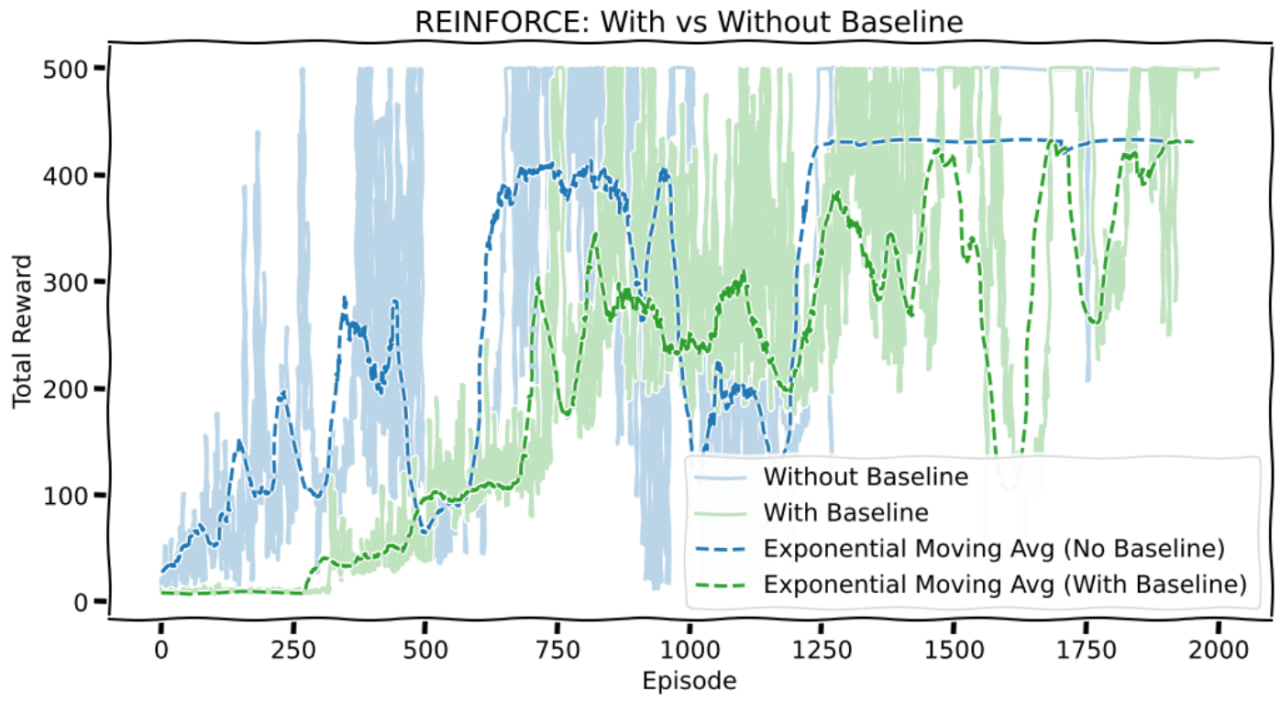
\includegraphics[width = 1\textwidth]{figs/baseline.jpg}
 \caption{comparison of REINFORCE with baseline and REINFOCE without baseline}
\end{figure}
As it is evident in the image, the baseline method has lower variance
\subsection{Question 6:}

Explain how variance affects policy gradient methods, particularly in the context of estimating gradients from sampled trajectories.
\\
High variance in policy gradient methods occurs because they estimate gradients from a limited number of sampled trajectories, which may not fully represent the true distribution of possible outcomes. This variance is amplified when rewards are sparse, delayed, or have high magnitude differences. As trajectory length increases, variance grows substantially because small differences in early actions can lead to vastly different returns. This excessive variance causes unstable updates where the policy might improve in one update but degrade in the next, resulting in erratic learning, slower convergence, or even failure to learn. Techniques like baselines, advantage functions, and multiple trajectory sampling help mitigate this issue by providing more reliable gradient estimates.

\newpage

\section{Task 3: REINFORCE in a continuous action space [20]}

\subsection{Question 1:}

How are the observation and action spaces defined in the MountainCarContinuous environment?
\vspace*{0.3cm}\\
Both are continous spaces.
\subsection{Question 2:}

How could an agent reach the goal in the MountainCarContinuous environment while using the least amount of energy? Explain a scenario describing the agent's behavior during an episode with most optimal policy.
\vspace*{0.3cm}\\
To reach the goal in the MountainCarContinuous environment while using the least amount of energy, an agent should learn to strategically oscillate back and forth between the slopes by applying small bursts of acceleration in both directions, effectively building up momentum to reach the top of the hill with minimal energy expenditure, essentially "swinging" the car to the goal rather than directly powering up the slope.
\subsection{Question 3:}

What strategies can be employed to reduce catastrophic forgetting in continuous action space environments like MountainCarContinuous?

(Hint: experience replay or target networks)
\vspace*{0.3cm}\\
Catastrophic forgetting is a challenge in continuous learning, especially in environments like MountainCarContinuous. Here are key strategies:

\begin{itemize}
    \item \textbf{Experience Replay:} Store and sample past experiences to break correlation and learn from diverse data.
    \item \textbf{Target Networks:} Use separate, less frequently updated networks for stable target value estimation.
    \item \textbf{Elastic Weight Consolidation (EWC):} Protect important weights by penalizing changes crucial for past tasks.
    \item \textbf{Regularization:} Use L1/L2 to prevent overfitting to recent experiences.
    \item \textbf{Reward Normalization:} Stabilize training with consistent reward scales.
\end{itemize}

These techniques, particularly experience replay and target networks, are crucial for mitigating forgetting in MountainCarContinuous.

\newpage

\section{Task 4: Policy Gradient Drawbacks [25]}

\subsection{Question 1:}
\textbf{Which algorithm performs better in the Frozen Lake environment? Why?}
\newline
Compare the performance of Deep Q-Network (DQN) and Policy Gradient (REINFORCE) in terms of training stability, convergence speed, and overall success rate. Based on your observations, which algorithm achieves better results in this environment?\\
\textbf{DQN:}
\begin{itemize}
    \item Stable in discrete spaces, less so in continuous.
    \item Variable convergence speed.
    \item Complex adaptation for continuous actions.
\end{itemize}

\textbf{REINFORCE:}
\begin{itemize}
    \item High variance, unstable training.
    \item Potentially slow convergence.
    \item Well-suited for continuous actions.
\end{itemize}

\textbf{Conclusion:} REINFORCE, and policy gradient methods in general, typically perform better in continuous action spaces due to direct policy optimization.

\subsection{Question 2:}
\textbf{ What challenges does the Frozen Lake environment introduce for reinforcement learning?}
\newline
Explain the specific difficulties that arise in this environment. How do these challenges affect the learning process for both DQN and Policy Gradient methods?\\

Frozen Lake presents:

\begin{itemize}
    \item \textbf{Stochasticity:} Slippery ice introduces randomness, making transitions unpredictable.
    \item \textbf{Sparse Rewards:} Only the goal state yields a positive reward, hindering learning.
    \item \textbf{Long-Term Dependencies:} Optimal paths require multiple steps, demanding credit assignment over extended sequences.
\end{itemize}

\textbf{Effects:}

\begin{itemize}
    \item \textbf{DQN:} Struggles with stochasticity and sparse rewards, leading to unstable Q-value estimates and slow learning.
    \item \textbf{Policy Gradient:} High variance due to stochasticity and difficulty in credit assignment due to sparse rewards and long term dependencies.
\end{itemize}

These challenges slow convergence and reduce learning efficiency for both methods. 
\subsection{Question 3:}
\textbf{For environments with unlimited interactions and low-cost sampling, which algorithm is more suitable?}
\newline
In scenarios where the agent can sample an unlimited number of interactions without computational constraints, which approach—DQN or Policy Gradient—is more advantageous? Consider factors such as sample efficiency, function approximation, and stability of learning.
\\
In environments with unlimited, low-cost interactions:

\begin{itemize}
    \item \textbf{Policy Gradient} methods become highly advantageous.
\end{itemize}

\textbf{Reasons:}

\begin{itemize}
    \item \textbf{Sample Efficiency Irrelevant:} With unlimited samples, low sample efficiency of policy gradients is no longer a major concern.
    \item \textbf{Direct Policy Optimization:} Policy gradients directly optimize the policy, potentially leading to better convergence in complex environments, given enough samples.
    \item \textbf{Function Approximation Flexibility:} While both methods use function approximation, policy gradients often demonstrate more stable behavior with complex function approximators when provided with abundant data.

\end{itemize}

\textbf{Conclusion:} When sampling is effectively free, the direct policy optimization of Policy Gradient methods offers a significant advantage.

}}


%%%%%%%%%%%%%%%%%%%%%%%%%%%%%%%%%%%%%%%%%%%%%%%%%

\newpage

{\fontfamily{lmss}\selectfont {\color{DarkBlue}

\begin{thebibliography}{9}

\bibitem{CoverImage}
Cover image designed by freepik. Available: \href{https://www.freepik.com/free-vector/cute-artificial-intelligence-robot-isometric-icon_16717130.htm}{https://www.freepik.com/free-vector/cute-artificial-intelligence-robot-isometric-icon\_16717130.htm}

\bibitem{PolicySearch}
Policy Search. Available: 
\url{https://amfarahmand.github.io/IntroRL/lectures/lec06.pdf}

\bibitem{CartPole}
CartPole environment from OpenAI Gym. Available: \url{https://www.gymlibrary.dev/environments/classic_control/cart_pole/}

\bibitem{MountainCar}
Mountain Car Continuous environment from OpenAI Gym. Available: \url{https://www.gymlibrary.dev/environments/classic_control/cart_pole/}

\bibitem{FrozenLake}
FrozenLake environment from OpenAI Gym. Available: \url{https://www.gymlibrary.dev/environments/toy_text/frozen_lake/}

\end{thebibliography}

%%%%%%%%%%%%%%%%%%%%%%%%%%%%%%%%%%%%%%%%%%%%%%%%%

\end{document}
